\documentclass{ti2}

\usepackage{listings}
\usepackage{tikz}
\usepackage{ulem}
\usepackage{tikz-timing}[2009/05/15]
\usepackage{graphicx}

% Dateikodierung ist utf8
\usepackage[utf8]{inputenc}   


\usetikzlibrary{matrix,arrows.meta}
\tikzset{
	box/.style = { font=\sffamily, fill=black!20, centered },
	arrow/.style = { very thick, color=black, ->, >=Triangle},
}

\begin{document}

%damit der Code nicht abgeschnitten wird, falls er zu lang ist.
\lstset{linewidth=\linewidth,breaklines=true}
% Nr, Abgabedatum, Gruppenleiter, Gruppenname, Name1...Name4
\Abgabeblatt{4}{28.11.2016}{Marc Hildebrandt}{C08}%
                {Timo Jasper (Inf, 3.FS.)}{Thomas Tannous (Inf, 3.FS.)}%
                {Moritz Gerken (Inf, 3.FS.)}%

\section*{Gruppe}
	Oliver Hilbrecht hat sich entschlossen TI2 in diesem Semester abzubrechen.\\

\section*{Aufgabe 1}
\lstinputlisting[language=C]{./src/ti2sh.cc}

Wir haben uns für den Signal Händler des Signals SIGCHLD entschieden. Dieser sorgt dafür das Hintergrundprozesse der Shell, sobald sie in den Zombie-Status wechseln, direkt aus der Prozess-Tabelle vom Parent entfernt werden.
Im Handler selbst wird waitpid mit  -1 aufgerufen was bedeutet, dass wait auf den Kindprozess warten soll. WNOHANG sorgt dafür, dass waitpid sofort returned, wenn kein Kind sich schließt. 
Um die Umgebungsvaribale PATH zu parsen, haben wir die extra Funktion getPathToExec geschrieben, welche aus einem command Namen, wie z.B. "ls" den Pfad zum binären Programm angibt, indem es alle Pfade, die in PATH enthalten ist durchläuft und mit access checkt, ob die Datei vorhanden ist. X\_OK checkt zu dem zusätzlich für executable permissions. Falls ein Programm nicht im Hintergrund laufen soll warten im Elternrprozess mit wait auf die Terminierung des Kindprozesses.

\subsection*{Tests}



Wir haben Tests entsprechend aller Anforderungen des Übungsblattes ausgeführt.\\
Wir haben verschiedene Kommandos mit verschieden vielen Parametern getestet.\\
Wir haben Prozesse im Vorder- und Hintergrund laufen lassen, zum teil Parallel.(sleep 10, während sleep 60 \& im Hintergrund läuft)\\
Wir haben Befehle mit absoluten Pfaden ausgeführt.\\
Verzeichnisswechsel d. Shellstatus war nicht erfolgreich, die Aufgabenstellung verlangt nur das arbeiten mit absoluten Pfaden, daher ist auch nicht relevant, welches Verzeichnis im Shell Status ist.\\
Das gleichzeitige ausführen mehrerer Kommandos mit einer Zeile wurde bereits als nicht implementiert vorgegeben.\\

\begin{tabular}{|l|l|l|}
	\hline
	Eingabe & Erw. Ausgabe/Reaktion & Ergbenis\\
	\hline
	ti2sh\$ ls & Inhalte aktuelles Verzeichnis & erfolgreich\\
	\hline
	ti2sh\$ ls -l & die selben Inhalte+weitere Infos in vertikaler Liste & erfolgreich\\
	\hline
	ti2sh\$ ls -l -i & nochmal das selbe + Inode Nummer & erfolgreich\\
	\hline
	ti2sh\$ echo Test & Ausgabe von "Test" & erfolgreich\\
	\hline
	ti2sh\$ sleep 60 \& & Prozess soll im Hintergrund laufen & erfolgreich\\
	\hline
	ti2sh\$ sleep 10 & Prozess sollte für 10sec im Vordergrund laufen & erfolgreich\\
	\hline
	ti2sh\$ cd ./src/ & Verzeichnis der Shell wechseln & nicht erfolgreich\\
	\hline
	ti2sh\$ evince $\sim$/home/.../ueb4.pdf & pdf anzeige d. 4 Übungsblattes & erfolgreich\\
	\hline
	ti2sh\$  sleep 5 \& jobs & Ausgabe des Kindprozesses (sleep) & nicht impl.\\
	\hline
	ti2sh\$ ctrl. + d & Shell schließt sich & erfolgreich\\
	\hline
\end{tabular}

\section*{Aufgabe 2}
%Ein gedachter Rechner verwendet den Buddy-Algorithmus zur Speicherverwaltung. Anfangs
%existiert ein Block mit 64,KiB (65536 Byte) ab Adresse 0. Gebt für die folgenden Speicheran-
%forderungen und ihre Auswirkungen jeweils eine Grafik analog zur Vorlesung bzw. Tutorium
%an:


\subsection*{2 a)}
%a) Nachdem aufeinanderfolgende Anforderungen für 10 KiB, 12 KiB, 3 KiB, 16 KiB, 1 KiB, 20
%KiB und 2 KiB eingetroffen sind: wieviele freie Blöcke bleiben übrig, was sind ihre Größen
%und Adressen?

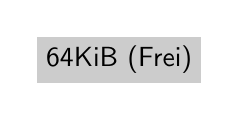
\begin{tikzpicture}
\matrix (m)
[
matrix of nodes,
column sep      = 1em,
row sep         = 1ex,
column 1/.style = { nodes = { box } },
column 2/.style = { nodes = { box } },
column 3/.style = { nodes = { box } },
column 4/.style = { nodes = { box } },
column 5/.style = { nodes = { box } },
column 6/.style = { nodes = { box } },
column 7/.style = { nodes = { box } },
]
{
	64KiB (Frei)\\
};
\end{tikzpicture}\\
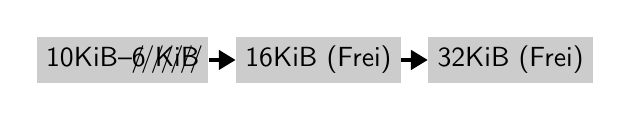
\begin{tikzpicture}
\matrix (m)
[
matrix of nodes,
column sep      = 1em,
row sep         = 1ex,
column 1/.style = { nodes = { box } },
column 2/.style = { nodes = { box } },
column 3/.style = { nodes = { box } },
column 4/.style = { nodes = { box } },
column 5/.style = { nodes = { box } },
column 6/.style = { nodes = { box } },
column 7/.style = { nodes = { box } },
]
{
	10KiB--\xout{6 KiB} & 16KiB (Frei) & 32KiB (Frei)\\
};
\foreach \i/\j in {1/2} {
	\draw [arrow] (m-\i-1) -- (m-\i-2);
	\draw [arrow] (m-\i-2) -- (m-\i-3);
}
\end{tikzpicture}\\
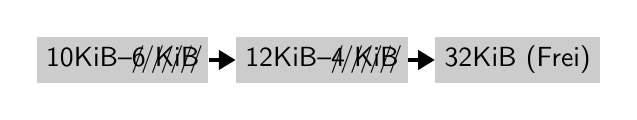
\begin{tikzpicture}
\matrix (m)
[
matrix of nodes,
column sep      = 1em,
row sep         = 1ex,
column 1/.style = { nodes = { box } },
column 2/.style = { nodes = { box } },
column 3/.style = { nodes = { box } },
column 4/.style = { nodes = { box } },
column 5/.style = { nodes = { box } },
column 6/.style = { nodes = { box } },
column 7/.style = { nodes = { box } },
]
{
	10KiB--\xout{6 KiB} & 12KiB--\xout{4 KiB} & 32KiB (Frei)\\
};
\foreach \i/\j in {1/2} {
	\draw [arrow] (m-\i-1) -- (m-\i-2);
	\draw [arrow] (m-\i-2) -- (m-\i-3);
}
\end{tikzpicture}\\
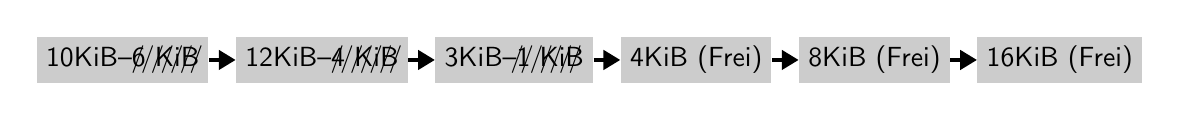
\begin{tikzpicture}
\matrix (m)
[
matrix of nodes,
column sep      = 1em,
row sep         = 1ex,
column 1/.style = { nodes = { box } },
column 2/.style = { nodes = { box } },
column 3/.style = { nodes = { box } },
column 4/.style = { nodes = { box } },
column 5/.style = { nodes = { box } },
column 6/.style = { nodes = { box } },
column 7/.style = { nodes = { box } },
]
{
	10KiB--\xout{6 KiB} & 12KiB--\xout{4 KiB} & 3KiB--\xout{1 KiB} & 4KiB (Frei) & 8KiB (Frei) & 16KiB (Frei)\\
};
\foreach \i/\j in {1/2} {
	\draw [arrow] (m-\i-1) -- (m-\i-2);
	\draw [arrow] (m-\i-2) -- (m-\i-3);
	\draw [arrow] (m-\i-3) -- (m-\i-4);
	\draw [arrow] (m-\i-4) -- (m-\i-5);
	\draw [arrow] (m-\i-5) -- (m-\i-6);
}
\end{tikzpicture}\\

\begin{tikzpicture}
\matrix (m)
[
matrix of nodes,
column sep      = 1em,
row sep         = 1ex,
column 1/.style = { nodes = { box } },
column 2/.style = { nodes = { box } },
column 3/.style = { nodes = { box } },
column 4/.style = { nodes = { box } },
column 5/.style = { nodes = { box } },
column 6/.style = { nodes = { box } },
column 7/.style = { nodes = { box } },
]
{
	10KiB--\xout{6 KiB} & 12KiB--\xout{4 KiB} & 3KiB--\xout{1 KiB} & 4KiB (Frei) & 8KiB (Frei) & 16KiB\\
};
\foreach \i/\j in {1/2} {
	\draw [arrow] (m-\i-1) -- (m-\i-2);
	\draw [arrow] (m-\i-2) -- (m-\i-3);
	\draw [arrow] (m-\i-3) -- (m-\i-4);
	\draw [arrow] (m-\i-4) -- (m-\i-5);
	\draw [arrow] (m-\i-5) -- (m-\i-6);
}
\end{tikzpicture}\\

\begin{tikzpicture}
\matrix (m)
[
matrix of nodes,
column sep      = 1em,
row sep         = 1ex,
column 1/.style = { nodes = { box } },
column 2/.style = { nodes = { box } },
column 3/.style = { nodes = { box } },
column 4/.style = { nodes = { box } },
column 5/.style = { nodes = { box } },
column 6/.style = { nodes = { box } },
column 7/.style = { nodes = { box } },
]
{
	10KiB--\xout{6 KiB} & 12KiB--\xout{4 KiB} & 3KiB--\xout{1 KiB} & 1KiB--\xout{3 KiB} & 8KiB (Frei) & 16KiB\\
};
\foreach \i/\j in {1/2} {
	\draw [arrow] (m-\i-1) -- (m-\i-2);
	\draw [arrow] (m-\i-2) -- (m-\i-3);
	\draw [arrow] (m-\i-3) -- (m-\i-4);
	\draw [arrow] (m-\i-4) -- (m-\i-5);
	\draw [arrow] (m-\i-5) -- (m-\i-6);
}
\end{tikzpicture}\\

\begin{tikzpicture}
\matrix (m)
[
matrix of nodes,
column sep      = 1em,
row sep         = 1ex,
column 1/.style = { nodes = { box } },
column 2/.style = { nodes = { box } },
column 3/.style = { nodes = { box } },
column 4/.style = { nodes = { box } },
column 5/.style = { nodes = { box } },
column 6/.style = { nodes = { box } },
column 7/.style = { nodes = { box } },
]
{
	10KiB--\xout{6 KiB} & 12KiB--\xout{4 KiB} & 3KiB--\xout{1 KiB} & 1KiB--\xout{3 KiB} & 2KiB--\xout{2 KiB} & 4KiB (Frei) & 16KiB\\
};
\foreach \i/\j in {1/2} {
	\draw [arrow] (m-\i-1) -- (m-\i-2);
	\draw [arrow] (m-\i-2) -- (m-\i-3);
	\draw [arrow] (m-\i-3) -- (m-\i-4);
	\draw [arrow] (m-\i-4) -- (m-\i-5);
	\draw [arrow] (m-\i-5) -- (m-\i-6);
	\draw [arrow] (m-\i-6) -- (m-\i-7);
}
\end{tikzpicture}

Die Anforderung von 20KiB kann nicht erfüllt werden, da zu dem Zeitpunkt bereits kein Block von außreichender Größe mehr Frei ist.\\

Der in der Abb. markierte Block mit der Größe 4KiB ist frei geblieben.
Die Adresse haben wir ermittelt, indem wir von der Adresse: 0 an, die Blockgrößen aufaddiert haben, bis zum Freien 4 KiB Block.
Der Freie Block befindet sich also an der Adresse: 45056.



\subsection*{2 b)}
%b) Anschließend werden die Blöcke für die Anforderungen 2 KiB, 16 KiB und 3 KiB wieder
%freigegeben. Welche Blöcke gibt es nun? Könnte eine folgende Anforderung von 21 KiB
%erfüllt werden?

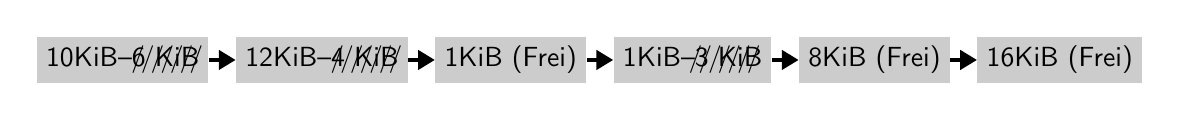
\begin{tikzpicture}
\matrix (m)
[
matrix of nodes,
column sep      = 1em,
row sep         = 1ex,
column 1/.style = { nodes = { box } },
column 2/.style = { nodes = { box } },
column 3/.style = { nodes = { box } },
column 4/.style = { nodes = { box } },
column 5/.style = { nodes = { box } },
column 6/.style = { nodes = { box } },
column 7/.style = { nodes = { box } },
]
{
	10KiB--\xout{6 KiB} & 12KiB--\xout{4 KiB} & 1KiB (Frei) & 1KiB--\xout{3 KiB} & 8KiB (Frei) & 16KiB (Frei)\\
};

\foreach \i/\j in {1/2} {
	\draw [arrow] (m-\i-1) -- (m-\i-2);
	\draw [arrow] (m-\i-2) -- (m-\i-3);
	\draw [arrow] (m-\i-3) -- (m-\i-4);
	\draw [arrow] (m-\i-4) -- (m-\i-5);
	\draw [arrow] (m-\i-5) -- (m-\i-6);
}

\end{tikzpicture}



Der Freigewordene 2KiB Block wird mit dem noch aus Aufgabe 2a) Freien 4 KiB Block verschmolzen und bilden einen 8 KiB Block, weitere Verschmelzungen sind nicht möglich.\\

Da der größte freie Block nur 16 KiB groß ist, kann die Anforderung von 21 KiB nicht erfüllt werden, außerdem muss auch noch die nicht erfüllte Anforderung von 20 KiB aus Aufgabe 2 a) berücksichtigt werden.\\

\section*{Aufgabe 3}


	%\includegraphics[width=30px\textwidth, height=30px]{image1.jpeg}
\includegraphics[scale=0.3, angle=90]{image1.jpeg}


%Stellt die Änderungen der Prozesshierarchie über die angegebene Zeit %grafisch dar wie im Tutorium
%gezeigt. Wann entstehen neue Prozesse, wann terminieren sie wieder? Wann %wird welchem Prozess
%welches Signal gesendet (und von wem)? Zu welchem Prozess gehört am Ende %das in Schritt 2
%gestartete Terminal?

Das Terminal von Schritt 2 gehört am Ende zum sleep Prozess.


\end{document}
